\chapter{引言}

\section{研究背景}

多机器人系统能够通过多个机器人之间的分工与协作完成单个机器人难以独立承担的任务，在灾害救援、海洋监测、仓储物流、交通巡检等场景中具有较高的应用价值。
其中，编队导航是多机器人协同控制中的典型问题，要求多个智能体在运动过程中保持特定的空间结构，并根据环境变化完成目标到达、障碍规避和队形维持等任务\cite{rawat2020multi,orr2023marl_multirobot_survey}。
在真实环境中，机器人需要面对动态障碍物、传感器噪声、通信延迟以及运动模型不确定等因素，机器人系统的安全性与合作协同能力往往会受到影响。

传统编队控制方法通常依赖较为精确的动力学模型和人工设计的控制规则，在环境结构清晰、扰动较弱的条件下能够取得稳定效果。
然而，当任务场景变得复杂后，方法的适应性和扩展性都会受到限制。
近年来，强化学习（Reinforcement Learning, RL）因具备从交互数据中学习复杂策略的能力，被逐渐用于多智能体协作与编队控制任务中\cite{罗彪2025多智能体强化学习控制与决策研究综述,gronauer2022multiagent_survey,yu2022surprising_mappo}。
借助与环境的反复交互，机器人能够在缺乏精确模型的条件下学到面向任务的协同行为，这正是强化学习被引入多机器人编队控制的主要动因。

当前，强化学习方法面临仿真到真实迁移的问题。多机器人策略通常先在高保真仿真环境中训练，再迁移到真实机器人或更接近真实系统的仿真平台中部署。
然而，仿真环境中的动力学参数、传感器噪声和障碍物信息很难完全等同于真实环境，策略在部署阶段可能出现性能下降。因此有必要在真实环境中进行训练与验证。因此保证机器人系统的安全是多机器人强化学习应用中必须解决的问题。
% 部分方法依赖精确动力学模型、在线障碍物感知或预设安全控制器来弥补这一差异，但这些先验条件在真实环境中并不容易获得。
% 对于资源受限的多机器人平台而言，实时计算复杂安全边界也会带来额外负担。

% 在机器人系统任务执行中，安全性问题尤其重要。

安全强化学习（Safe Reinforcement Learning, SafeRL）通常将上述问题建模为约束马尔可夫决策过程（Constrained Markov Decision Process, CMDP），
试图在优化累积回报的同时限制策略对安全约束的违反。但现有方法中，许多算法主要通过代价函数、拉格朗日乘子或惩罚项来调节策略行为，其约束满足往往具有软约束特征，
对超参数较为敏感，难以在训练全过程中持续保证安全\cite{gu2024review,zhao2023statewise_safe_survey,ray2019benchmarking,ji2024omnisafe,hsu2024safety_filter}。

此外，编队任务需要同时满足机器人间距、障碍物规避等多类约束。
若仅依靠奖励函数对这些约束进行间接惩罚，策略在训练或执行过程中仍可能产生不安全动作、队形破坏等问题。
% 多机器人场景中的风险还会进一步放大：单个机器人的动作变化可能影响邻近机器人，局部约束违背也可能传递为整体编队的不稳定。
% 因此，如何在策略学习过程中显式处理安全约束，是多机器人强化学习应用中必须解决的问题。

因此，本文的问题场景如图~\ref{fig:background}所示，即不确定环境中，要求多机器人完成编队任务的同时满足安全约束并保持稳定协同。为此，有必要构建一种兼顾安全约束、编队协同和部署可行性的策略学习方法，使机器人在不确定环境下能够保持较稳定的安全行为。

\begin{figure}[h]
    \centering
    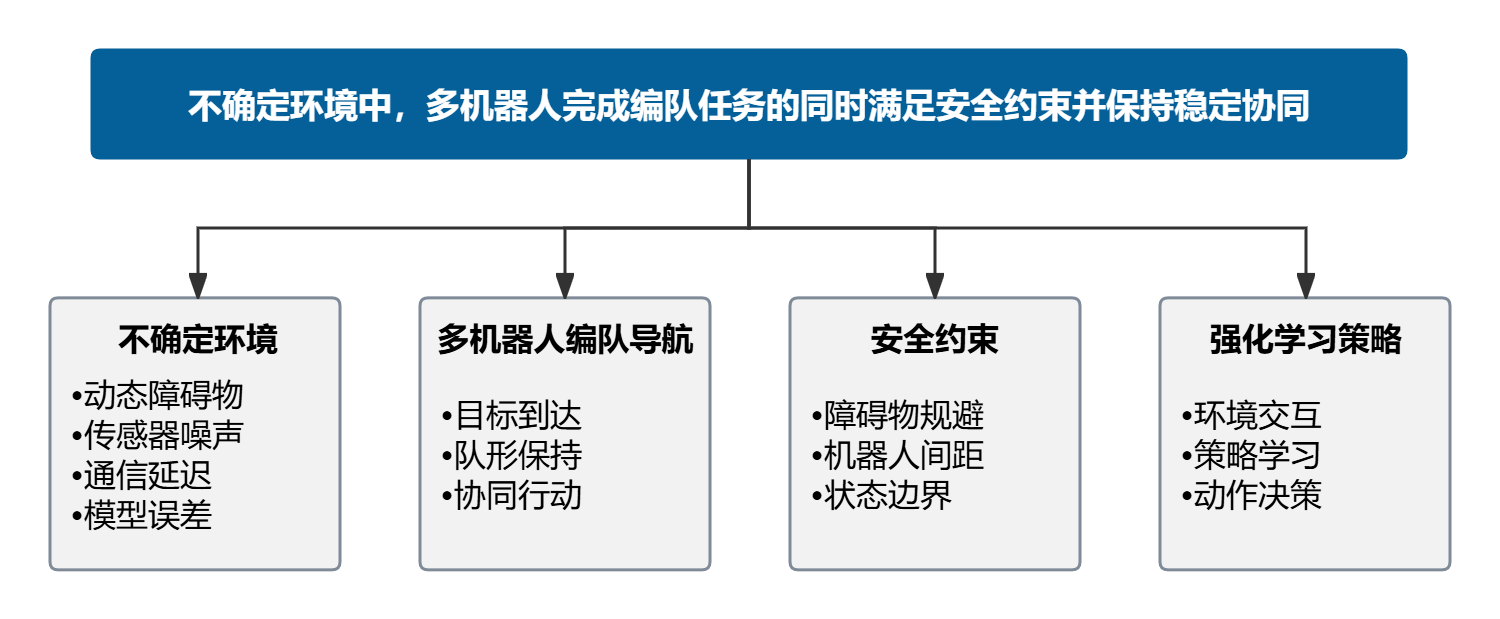
\includegraphics[width=0.8\textwidth]{images/background.png}
    \figcap{问题场景}{Problem scenario.}
    \label{fig:background}
\end{figure}

基于上述背景，本文围绕不确定环境下多机器人安全强化学习问题展开研究，重点关注三个方面：
一是利用约束流形与可达性分析对策略动作进行安全修正，减少训练和执行过程中的约束违背；
二是在多机器人编队导航任务中引入几何约束机制，使编队结构保持、安全距离约束和任务动作生成能够在统一框架下协同工作；
三是构建容器化仿真验证平台，为不同安全强化学习算法提供一致的运行环境和评估流程，从而验证所提方法在复杂场景中的有效性与可扩展性。

\section{研究意义}

多机器人系统在复杂环境中执行任务时，策略性能并不是唯一目标。对于编队导航这类任务而言，机器人既要到达目标区域，又要保持队形结构、避免碰撞，并在传感器噪声、障碍物变化和通信受限等条件下维持稳定运行。因此，如何在强化学习策略优化过程中同时处理任务收益和安全约束，是多机器人系统走向实际应用时必须面对的问题。本文围绕不确定环境下的多机器人安全强化学习展开研究，将约束流形、可达性分析、状态估计和几何约束机制引入策略学习过程，目的在于减少策略训练与执行中的约束违背，使学习得到的控制策略不仅具有较好的任务表现，也具备更稳定的安全边界。

在方法层面，本文把安全约束从奖励函数中的软惩罚移到了动作执行环节。多数安全强化学习方法用代价约束或拉格朗日乘子调节策略，其约束满足依赖超参数、且往往只在训练收敛后才较可靠，训练过程中仍可能违约；本文改用安全过滤、离线可达空间与奖励校准，把约束直接作用于动作的生成与修正，使不安全动作能在执行前被拦截。对编队导航中任务目标、安全距离与队形相互耦合的情形，几何约束策略学习进一步用几何关系而非奖励来修正策略输出，为提升多智能体方法的安全性与可解释性提供了一条区别于纯奖励塑形的途径。

在应用层面，仓储物流、灾害救援、巡检监测等场景中的多机器人往往要在动态环境下长时间运行，一次碰撞或队形失稳就可能中断任务甚至损坏设备，单纯追求任务效率并不够。本文实现的容器化仿真验证平台把运行依赖固化在镜像中，提供统一的算法接口与评估流程，缩小训练与部署环境之间的差异，也让不同算法能在相同条件下复现和比较，便于安全方法在进入实机前完成验证。

\section{研究内容}
本文研究不确定环境下的多机器人安全强化学习。与单纯的任务策略学习不同，这里的难点在于：训练阶段的试错探索本身就可能产生碰撞与队形破坏；而策略通常先在仿真中训练、再迁往实机，仿真与现实之间的动力学差异和传感器噪声又会削弱其可靠性。围绕这一难点，研究内容沿"安全动作约束—编队协同策略—系统验证平台"三条主线展开，力求在保证安全的前提下提升任务执行效率与部署可行性。技术路线如图~\ref{fig:tech_route}所示。

\begin{figure}[h]
    \centering
    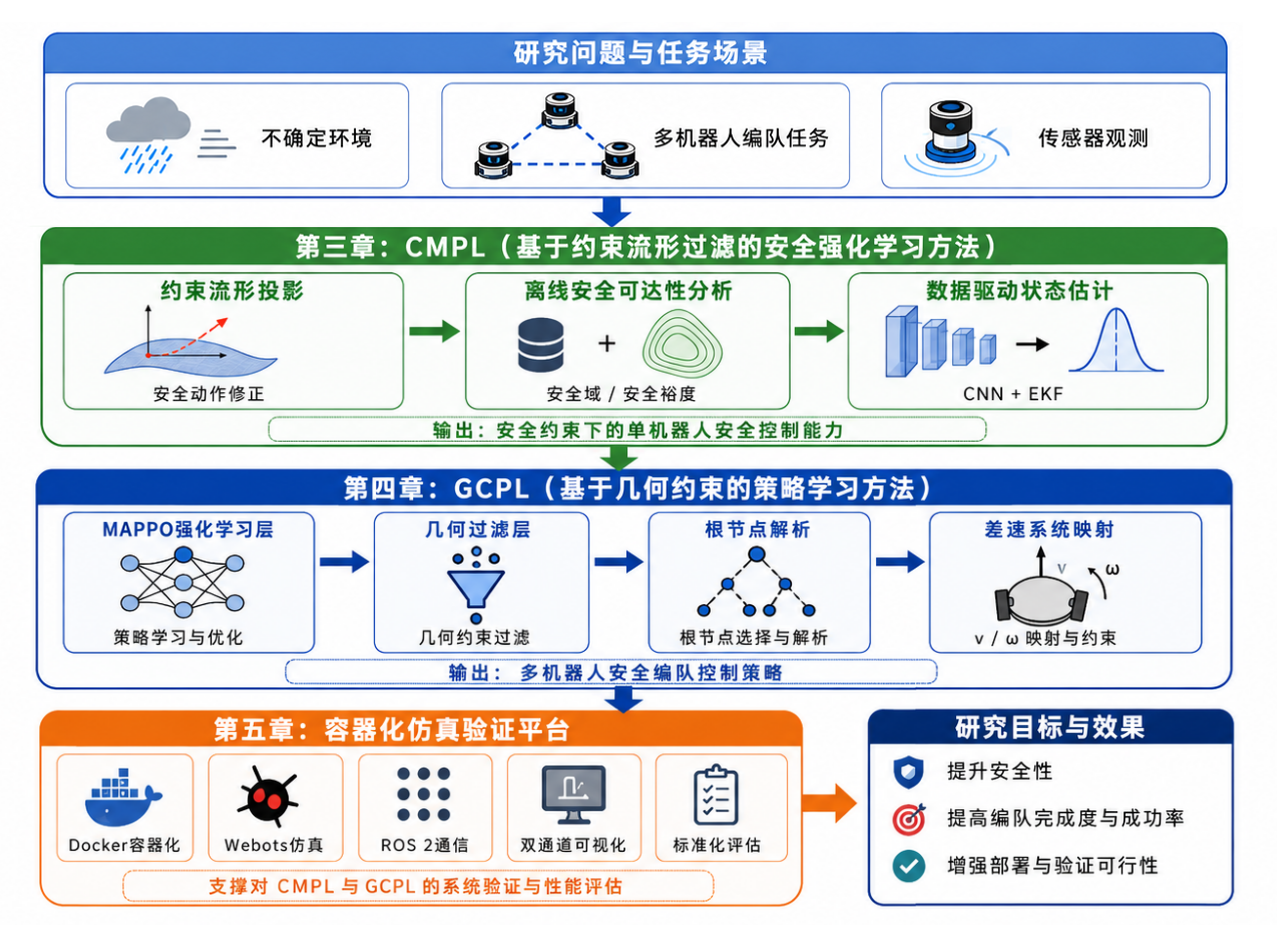
\includegraphics[width=0.8\textwidth]{images/tech_route.png}
    \figcap{技术路线}{Technical route.}
    \label{fig:tech_route}
\end{figure}


\textbf{（1）构建基于约束流形与可达性分析的安全策略修正方法}：传统强化学习算法主要通过与环境反复交互来最大化累积奖励，通常不会在动作生成阶段显式保证安全约束。已有安全强化学习方法虽然引入了代价约束或惩罚机制，但多数仍属于软约束形式，约束满足效果容易受到惩罚权重和训练状态的影响，在动态环境和感知噪声条件下难以稳定实现低违约甚至零违约表现。针对这一问题，本文引入约束流形思想，将机器人与障碍物之间的安全距离、状态边界等约束转化为增广状态空间中的流形约束，并通过零空间投影对策略输出的原始动作进行修正，使最终执行动作尽量保持原策略意图，同时满足安全可行条件。在此基础上，本文结合离线可达性分析，利用环境先验和采样轨迹构建安全可达空间，使安全裕度能够随机器人运动状态和环境风险变化进行调整。考虑到传感器噪声会影响安全判断的准确性，本文进一步引入数据驱动的状态估计模块，对速度相关噪声条件下的测量协方差进行自适应建模，从而为安全过滤器提供更可靠的状态输入。

\textbf{（2）提出面向多机器人编队导航的几何约束策略学习方法}：多机器人编队导航任务中，任务目标、安全约束和队形保持并不是彼此独立的要求。机器人在向目标移动时，需要根据邻近机器人和障碍物的位置不断调整自身动作；仅依赖奖励函数对队形偏差或碰撞风险进行惩罚，策略学习过程往往会出现收敛不稳定、局部行为不协调等问题。针对这一特点，本文在多智能体强化学习框架下构建基于几何约束的策略学习方法，以 MAPPO 生成任务驱动的动作，并在动作执行前引入几何过滤机制，对编队结构保持、机器人间安全距离和障碍物规避等约束进行统一处理。该方法利用约束流形和几何关系对策略输出进行修正，使多机器人系统在执行任务的同时维持较稳定的编队结构。

\textbf{（3）设计并实现多机器人安全强化学习的容器化仿真验证平台}：针对强化学习训练环境与部署环境的问题，本文设计并实现一套面向多机器人安全强化学习的容器化仿真验证平台。平台采用分层架构，通过容器化技术统一运行依赖，减少不同实验配置之间的环境差异。同时，平台提供标准化接口，并接入安全过滤器及多机器人协同策略。此外平台围绕安全性、任务性能、编队一致性和运行稳定性等指标构建评估流程，用于比较不同方法在相同场景下的表现。通过该平台，本文将前述安全约束机制与多机器人编队策略进行集成验证，从系统层面分析所提方法在复杂任务中的有效性、可扩展性和工程部署可行性。
